\section{Experiments}
\label{sec:experiments}

Our experiments examine the following hypotheses:\\
1. \textsc{cdl} can infer the causal graph, with less tuning and better accuracy than a regularization-based method \cite{wang2021task} (Sec. \ref{subsubsec:causal_graph_accuracy_results}).\\
2. Causal models learned by \textsc{cdl} generalize better than dense models in both dynamics and downstream task learning on unseen states (Sec. \ref{subsubsec:prediction_results}).\\
3. The transition collection policy learned by \textsc{cdl} improves the accuracy of causal dynamics learning compared to a uniform policy or the policy learned from the curiosity reward \cite{pathak2017curiosity}. (Sec. \ref{subsec:data_collection_policy_results}).\\
4. State abstractions derived by \textsc{cdl} improve sample-efficiency when learning downstream tasks compared to dense models which use the full state space (Sec. \ref{subsec:task_results}).\\
5. Policies learned by \textsc{cdl} for downstream tasks generalize better than those learned by dense models (Sec. \ref{subsec:task_results}).

\subsection{Environments}
\label{subsec:environment}

\begin{figure}
  \centering
  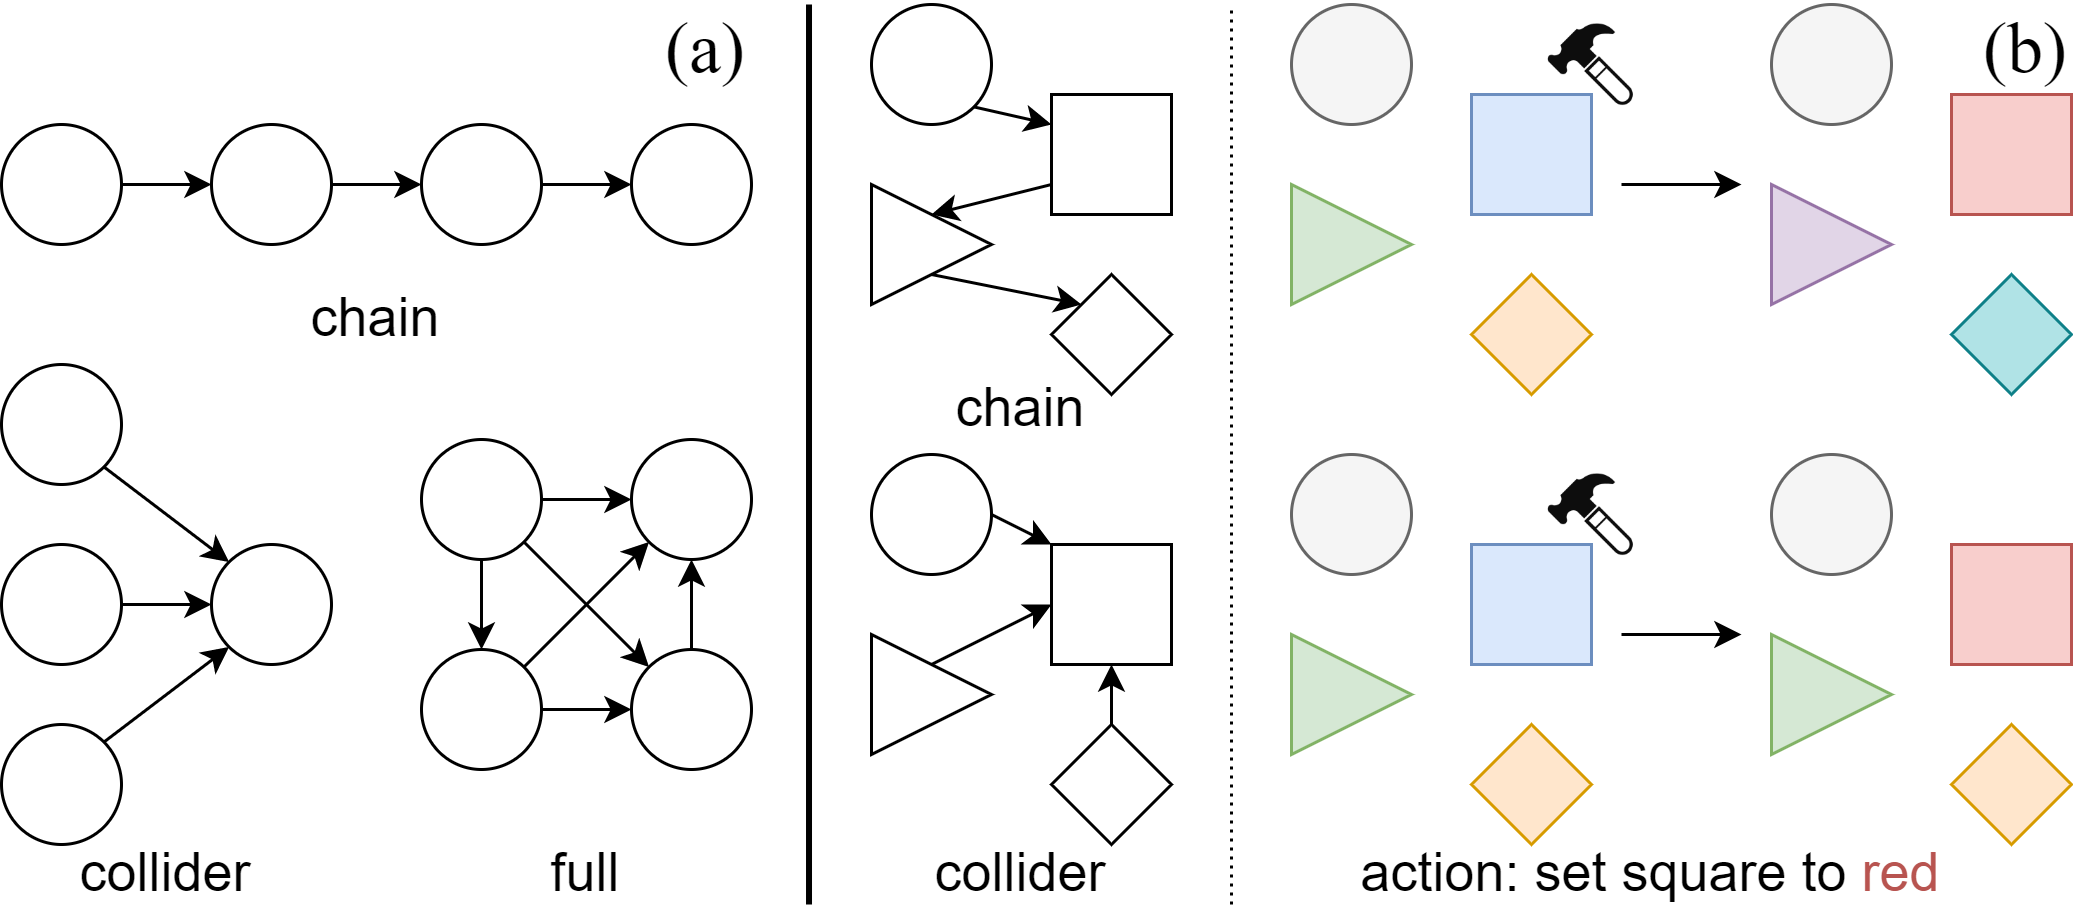
\includegraphics[width=0.9\columnwidth]{contents/figures/chemical.png}
  \vspace{-10pt}
  \caption{\small (a) different types of causal graphs. (b) illustration of the chemical environment (left: ground truth causal graphs, right: transitions after applying the action).}
  \label{fig:chemical_env}
  \vspace{-10pt}
\end{figure}

\begin{figure}
  \centering
  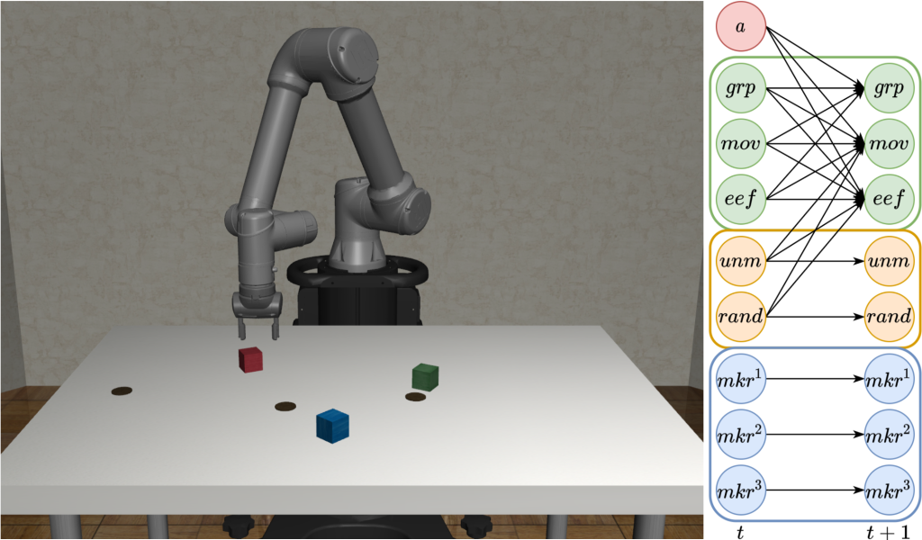
\includegraphics[width=0.9\columnwidth]{contents/figures/robosuite.png}
  \vspace{-10pt}
  \caption{\small \textbf{(Left)} the manipulation environment. \textbf{(Right)} the learned causal graph in the object level which recovers the ground truth relationship between the state variables and the action.}
  \label{fig:robosuite}
  \vspace{-15pt}
\end{figure}

We use (1) the Chemical environment modified from \citet{ke2021systematic} (Fig. \ref{fig:chemical_env} (b)) to examine \textsc{cdl}'s performance on causal graphs with different complexities, and (2) a manipulation environment (Fig. \ref{fig:robosuite}) to validate \textsc{cdl} with complex rigid-body dynamics.

In the chemical environment, there are 10 objects whose x,y positions are continuous and whose colors are one of 5 colors; the action can change a chosen object to a specified new color. The interactions between objects take place according to the underlying causal graph - when one object is set to a new color, all its descendants change their colors in the order of the graph following a predefined conditional probability table. The dynamics of colors and positions is independent for all objects: positions are sampled from a normal distribution every step. We consider three graph structures shown in Fig. \ref{fig:chemical_env} (a): full, chain, and collider.

In the manipulation environment implemented with the \texttt{robosuite} simulation framework \cite{robosuite2020}, there are three objects that the robot can interact with: a \textit{movable} red cube that the robot can manipulate (denoted as $mov$), an \textit{unmovable} green cube that is fixed on the table ($unm$), and a \textit{randomly moving} blue cube that also cannot be moved ($rand$). The purpose of the randomly moving object is to test whether \textsc{cdl} can learn that its motion is not caused by the robot's actions. There are also three randomly moving non-interactable markers ($mkr^1$, $mkr^2$, and $mkr^3$) on the table, as distractors to introduce potential spurious correlations. The state space consists of the robot end-effector (\textsc{eef}) location ($\mathbb{R}^3$), gripper ($grp$) joint angles ($\mathbb{R}^2$), and locations of objects and markers ($6 \times \mathbb{R}^3$). The action space includes \textsc{eef} location displacement ($\mathbb{R}^3$) and the degree to which the gripper is opened ($[0, 1]$). In each episode, the objects and markers are reset to randomly sampled poses on the table.

\subsection{Implementation}

\subsubsection{baselines}

We compare \textsc{cdl} with the following baselines:\\
1. \textbf{Reg}: regularization-based causal dynamics learning \cite{wang2021task}, where the causal mask $M$ is learned as trainable parameters rather than inferred from \textsc{cmi}.\\
2. \textbf{Modular}: using a separate network to predict each state variable \cite{ke2021systematic}, which can be represented by our method when none of the features are masked.\\
3. \textbf{GNN}: a graph neural network, following \cite{ke2021systematic}, we consider the C-SWM model \cite{kipf2019contrastive} which assumes dense dependence for each state variable.\\
4. \textbf{Monolithic}: a multi-layer perceptron (MLP) network that takes all state variables and actions as inputs and predicts the next step values of all state variables, which is commonly used in \textsc{mbrl}.

For a fair comparison, we use the same architecture for \textsc{cdl}, Reg, and Modular. For GNN and Monolithic whose architectures are different from the others, we try our best to give them the same number of parameters as others. See architectures of all methods in appendix Sec. \ref{app:architectures}.

\subsubsection{Causal Dynamics Learning}

We use MLP networks for feature extractors $f^a_{1:\dS}, f^{ 1:\dS}_{1:\dS}$ and predictive networks $q_{1:\dS}$. For continuous state variable $s^j_{t+1}$, $q_j$ outputs the mean and standard deviation of a normal distribution. For discrete state variable, $q_j$ outputs the logits of a categorical distribution. The threshold to infer causal relationships from \textsc{cmi} varies across environments.  We specify it along with other hyperparameters in appendix Sec. \ref{app:dynamics_learning}. Empirically, we find that reducing the frequency of optimizing causal prediction likelihood (i.e., $\log\hat{p}(s^j_{t+1} | \textbf{PA}_{s^j})$ in Eq. \ref{eq:dynamics_loss}) can stabilize training, so we only include this term once every 10 updates of the dynamics parameter $\theta$ according to Eq. \ref{eq:dynamics_loss} .

\subsubsection{Transition Collection Policy}

For the simple chemical environment, we use a random policy to collect transitions as it is enough to cover most of the state-action pairs. For the manipulation environment, we use Proximal Policy Optimization (PPO, \citet{schulman2017proximal}) as our RL agent. Meanwhile, as exploring the whole state space for manipulation domains is still a challenging research topic and not the focus of this paper, to reduce the complexity of exploration, we follow \citet{nasiriany2021maple} and modify PPO's action space to long-horizon skills, such as position reaching and object grasping/pushing (details in appendix Sec. \ref{app:transition_collection_policy_implementation}). Notice that dynamics learning still uses low-level raw motor actions described in Sec. \ref{subsec:environment}.

\subsection{Causal Dynamics Learning Evaluation}
\label{subsec:dynamics_results}

After training all methods on the same set of collected transition data (details in appendix Sec. \ref{app:transition_collection_policy_implementation}), we evaluate the quality of their learned dynamics in the following aspects:

\textit{Causal Relationship Inference}. We compare the causal graph inferred by \textsc{cdl} and Reg with the ground truth graph, in terms of edge accuracy.\\
\textit{Predicting Future States}. Given the current state and a sequence of actions, we evaluate the accuracy of each method's $k$-step prediction, for states both in and out of the training distribution (denoted as ID and OOD states). For the chemical environment, we evaluate color prediction in terms of mean accuracy (MA). For manipulation, log-likelihoods is used.\\
We also provide results using other metrics in the appendix Sec. \ref{app:dynamics_results}.

In the remainder of the paper, the performances shown for each method are mean and standard deviation computed from 3 models with different seeds.

\subsubsection{Causal Relationship Inference}
\label{subsubsec:causal_graph_accuracy_results}

\begin{table}
\centering
\caption{Causal Graph Accuracy (in $\%$) for \textsc{cdl} and Reg}
\vspace{-0pt}
\begin{small}
\begin{tabular}{ccc}
\toprule
\textbf{Environment} & \textbf{\textsc{cdl}} (Ours) & \textbf{Reg} \\
\midrule
Chemical (Collider) & \textbf{100.0} $\pm$ 0.0  & 99.4 $\pm$ 0.4 \\
Chemical (Chain)    & \textbf{100.0} $\pm$ 0.1  & 99.7 $\pm$ 0.1 \\
Chemical (Full)     & \textbf{99.1} $\pm$ 0.1   & 97.7 $\pm$ 0.4 \\
Manipulation        & \textbf{90.2} $\pm$ 0.3   & 84.4 $\pm$ 0.5 \\
\bottomrule
\end{tabular}
\end{small}
\vspace{-10pt}
\label{tab:causal_graph_accuracy}
\end{table}

As shown in Table. \ref{tab:causal_graph_accuracy}, in all environments, \textsc{cdl} learns the causal graph more accurately than Reg. Other baselines are not compared as they do not learn causal relationships. Fig. \ref{fig:robosuite} right shows the causal graph learned by \textsc{cdl} for the manipulation environment in the object level, and other quantitative and qualitative results can be found in appendix Sec. \ref{app:causal_graph_results} which collectively indicate that  \textsc{cdl} learns both fewer false positives (i.e., spurious correlations) and false negatives (i.e., missing necessary dependencies).

\subsubsection{Predicting Future States}
\label{subsubsec:prediction_results}

\begin{figure}
  \centering
  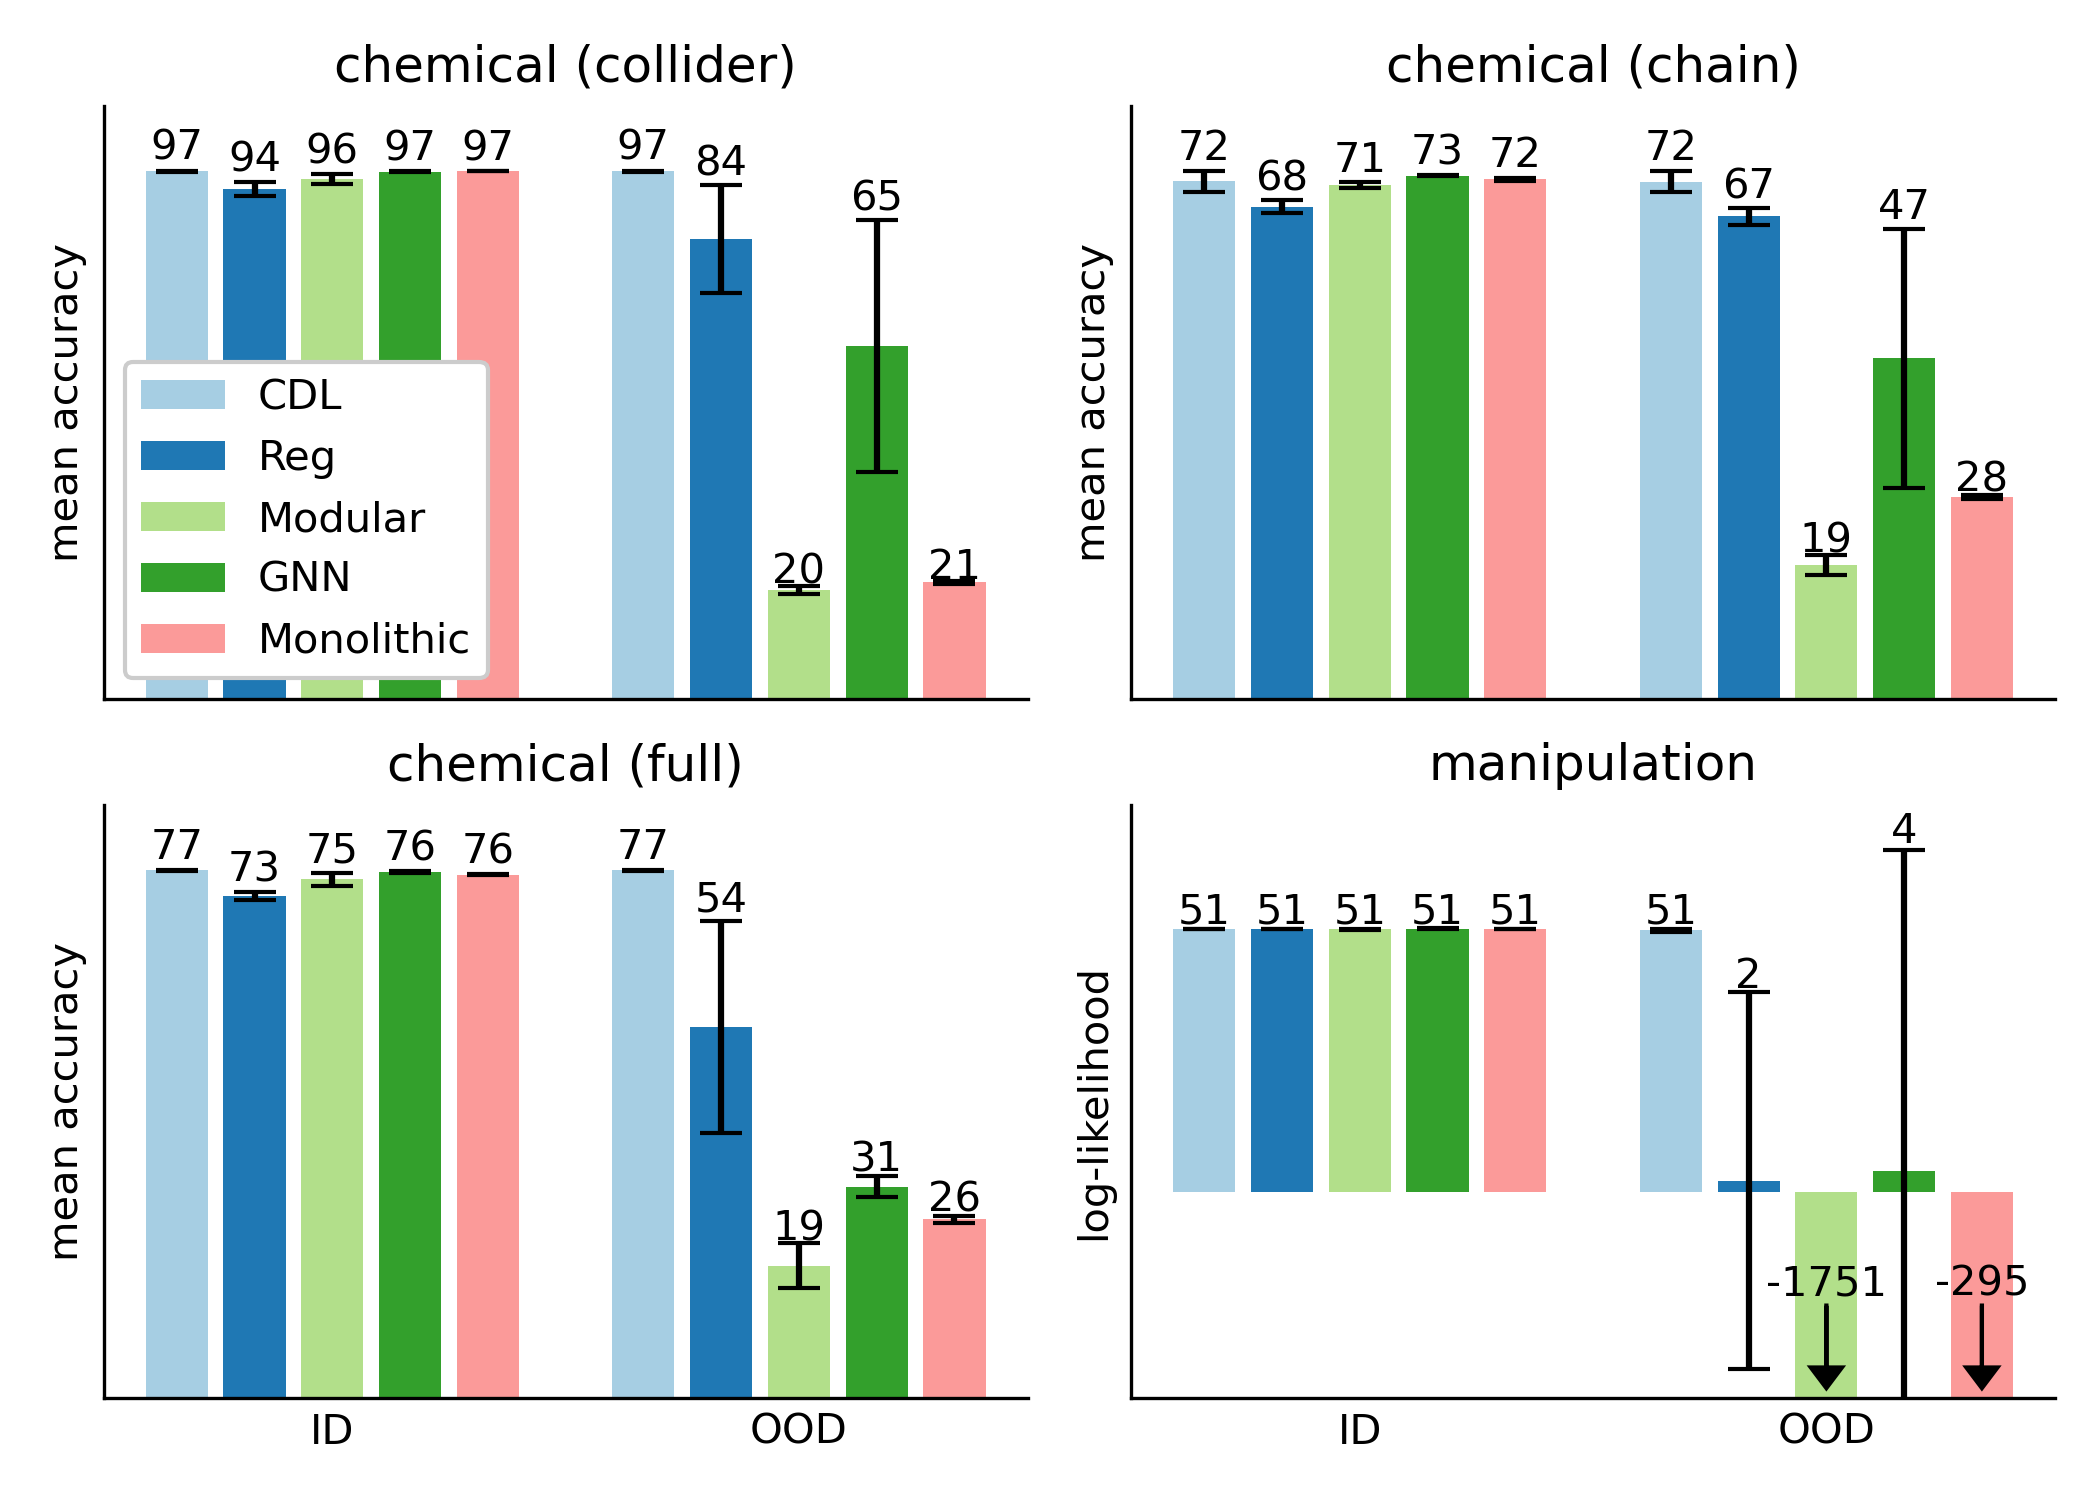
\includegraphics[width=1.0\columnwidth]{contents/figures/prediction.png}
  \vspace{-25pt}
  \caption{\small 1-step prediction performance on ID and OOD states. The mean is marked on top of each bar.}
  \label{fig:prediction_results}
  \vspace{-15pt}
\end{figure}

We evaluate each method for $1 \sim 5$-step prediction on 5K transitions, for both ID and OOD states. To create OOD states, we change object positions in the chemical environment and marker positions in the manipulation environment to unseen values, and the prediction is measured on other unchanged state variables. The 1-step prediction performance for each method is shown in Fig. \ref{fig:prediction_results} (the Modular and Monolithic in the bottom right plot are cropped due to their bad performances, and their means are labeled instead), and results for $2 \sim 5$-steps are in appendix Sec. \ref{app:prediction_results}. For ID states, all methods show similar prediction performance. However, for OOD states, the performance of dense models drops significantly as they suffer from spurious correlations while \textsc{cdl} and Reg mask those out with the learned dependencies. However, Reg also performs badly in the manipulation domain, because the trade-off between prediction accuracy and regularization leads to an inaccurate causal graph.


\subsection{Transition Collection Policy Learning Evaluation}
\label{subsec:data_collection_policy_results}

\begin{table}
\centering
\begin{small}
\caption{Causal Graph Accuracy for \textsc{cdl} with Different Transition Collection Policies}
\begin{tabular}{cccc}
\toprule
\textbf{Method}             & \textbf{PredDiff} (Ours) & \textbf{Uniform} & \textbf{Curiosity} \\
\midrule
\textbf{Accuracy} $(\%)$    & \textbf{90.2} $\pm$ 0.3 & 89.1 $\pm$ 0.6 & 88.9 $\pm$ 0.2 \\
\bottomrule
\end{tabular}
\end{small}
\vspace{-20pt}
\label{tab:policy_results}
\end{table}

To evaluate the benefits of the proposed transition collection policy (denoted as \textbf{PredDiff}), we compare its performance with the following methods, in terms of causal graph accuracy in the manipulation environment, \\
\textbf{Uniform}: a fixed policy that uniformly selects between skills and skill parameters instead of active exploration;\\
\textbf{Curiosity}: a policy that uses the prediction error of the causal predictor $\hat{p}(s^j_{t+1} | \textbf{PA}_{s^j})$ as rewards which encourages transitions where prediction errors are high \cite{pathak2017curiosity};

Table \ref{tab:policy_results} shows the accuracies of the causal graphs learned by \textsc{cdl} from the same amount of data (1.8M transitions) but collected by those three different policies, measured in the same way as Sec. \ref{subsubsec:causal_graph_accuracy_results}. Our PredDiff policy learns the graph with the highest accuracy. Though the accuracy differences between methods seem small, in a causal graph representing complex rigid body dynamics with $23 \times 24$ potential dependencies, $1\%$ accuracy difference means prediction errors for 5 $\sim$ 6 edges, which may severely harm the generalizability of the learned causal dynamics model. Furthermore, as shown in appendix Sec. \ref{app:data_collection_policy_results}, causal graphs learned by Uniform have more spurious correlations as it doesn't actively explore transitions where the causal graph is not learned well, and the Curiosity policy suffers from procrastination (i.e., repeats the transition with large stochasticity to maximize rewards) and fails to expose other causal dependencies. 

\subsection{Downstream Tasks Learning Evaluation}
\label{subsec:task_results}

We evaluate each method with the following downstream tasks in the chemical environment (C) and in the manipulation environment (M): \\
\textbf{Match} (C): match the object colors with goal colors individually, \\
\textbf{Reach} (M): move the end-effector to the goal position, \\
\textbf{Lift} (M): lift the movable object to the goal position,\\
\textbf{Stack} (M): stack the movable object on the top of the unmovable object.

The tasks' reward functions are unknown to the agent and are specified in appendix Sec. \ref{app:task_results}. During training, the dynamics model is frozen and only the reward predictor is learned as described in Sec. \ref{subsec:task_learning}.

\begin{figure}
  \centering
  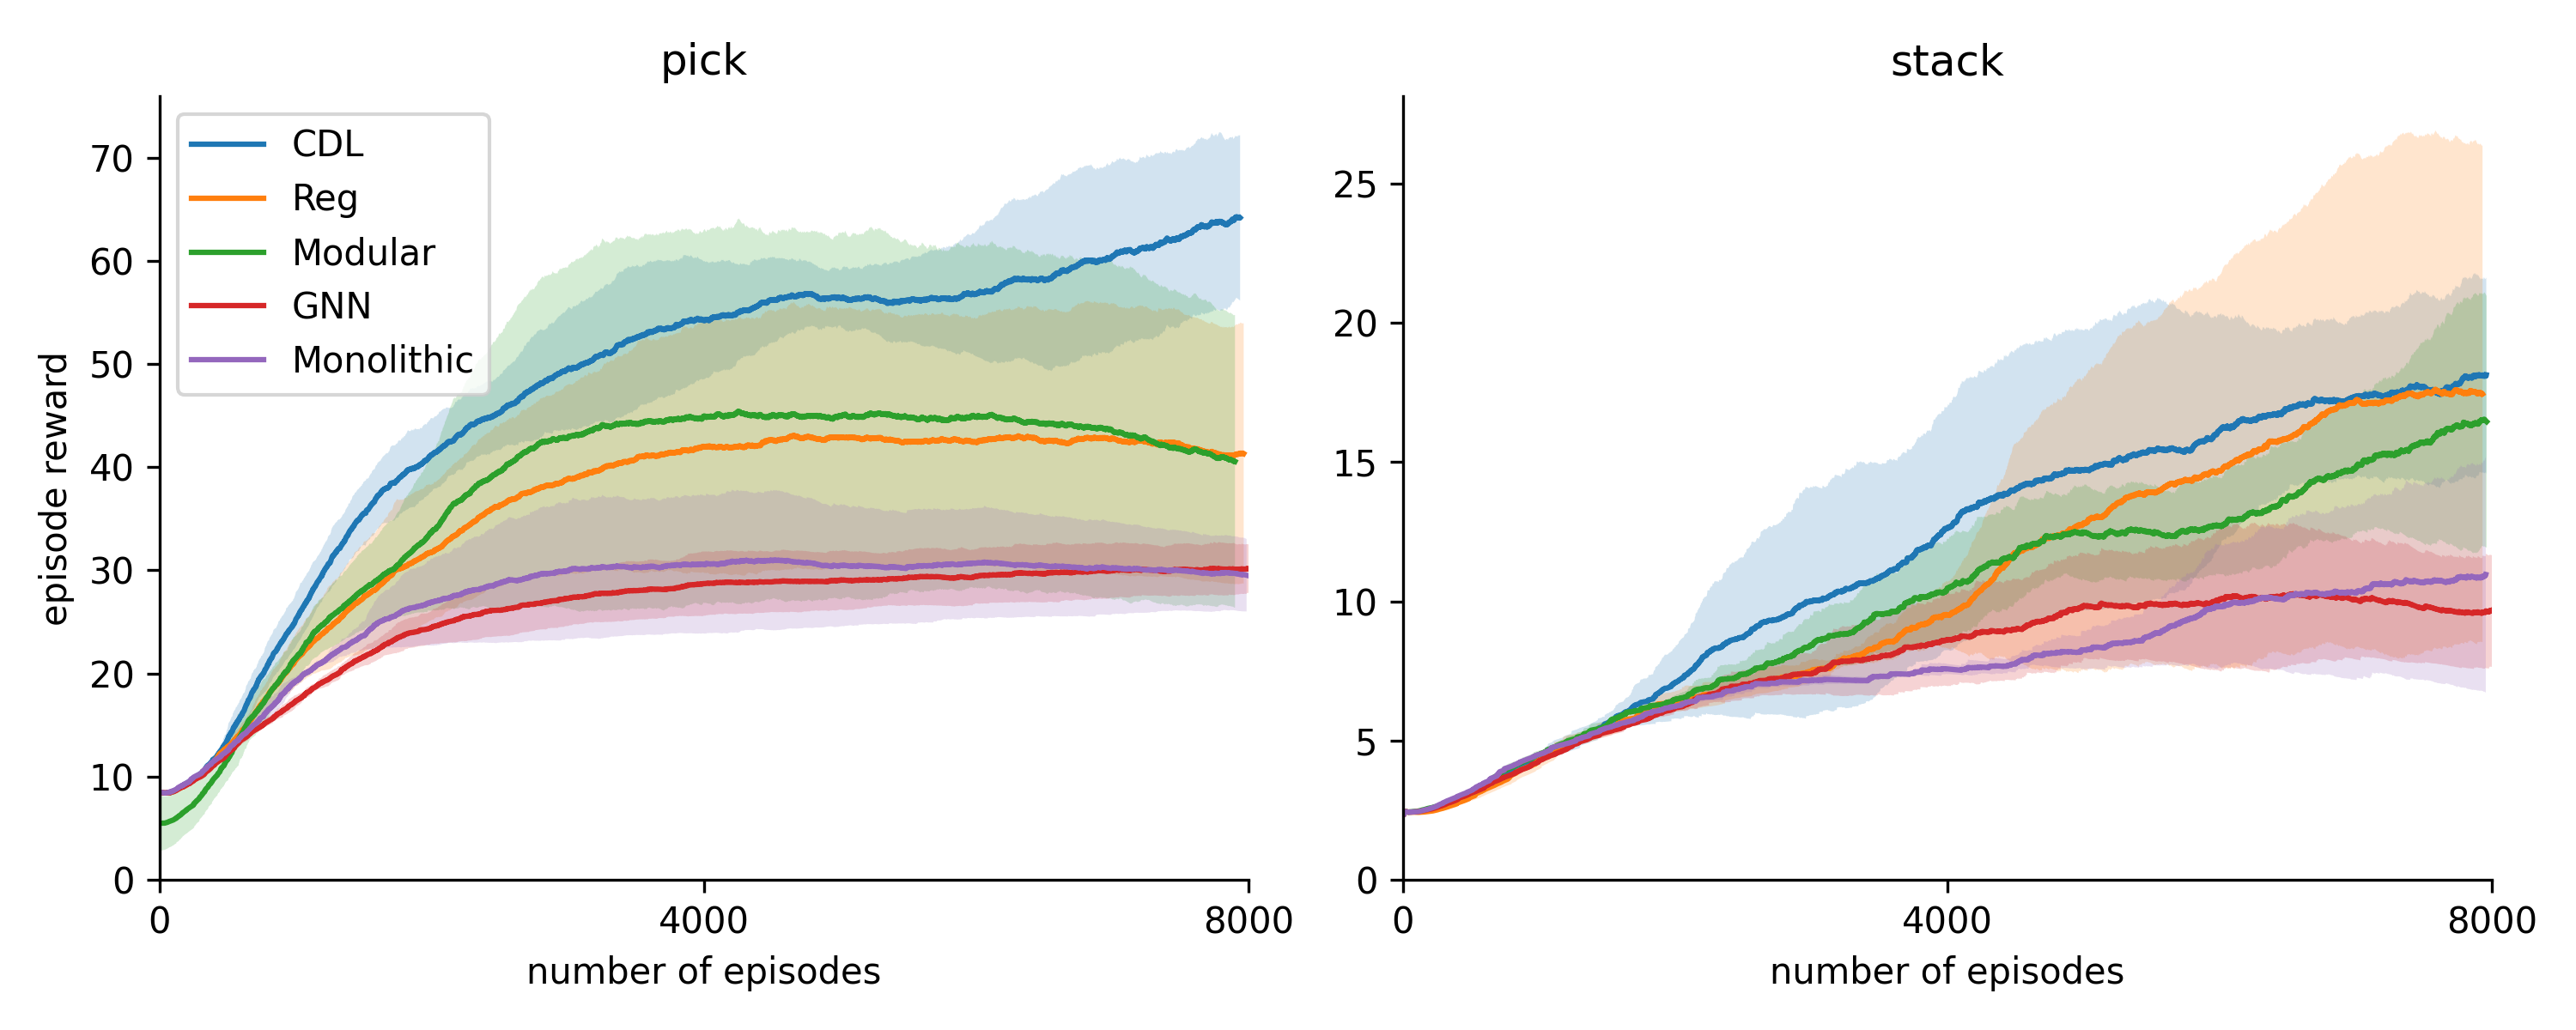
\includegraphics[width=1.0\columnwidth]{contents/figures/learning_curve.png}
  \vspace{-25pt}
  \caption{\small Training curves for two downstream tasks.}
  \label{fig:learning_curve}
  \vspace{-10pt}
\end{figure}

Compared to dense baselines, \textsc{cdl} and Reg also learn a causal graph so that they can learn tasks with the state abstraction described in Sec. \ref{subsec:problem_definition}. Fig. \ref{fig:learning_curve} shows the training curves of the Lift and Stack tasks (those of other tasks are in appendix Sec. \ref{app:task_results}); \textsc{cdl} learns tasks the most sample-efficiently with the state abstraction. Though Reg also uses abstraction, it learns more slowly as some action-irrelevant state variables are also included in the abstraction because of the inaccurately learned causal graphs.

\begin{figure}
  \centering
  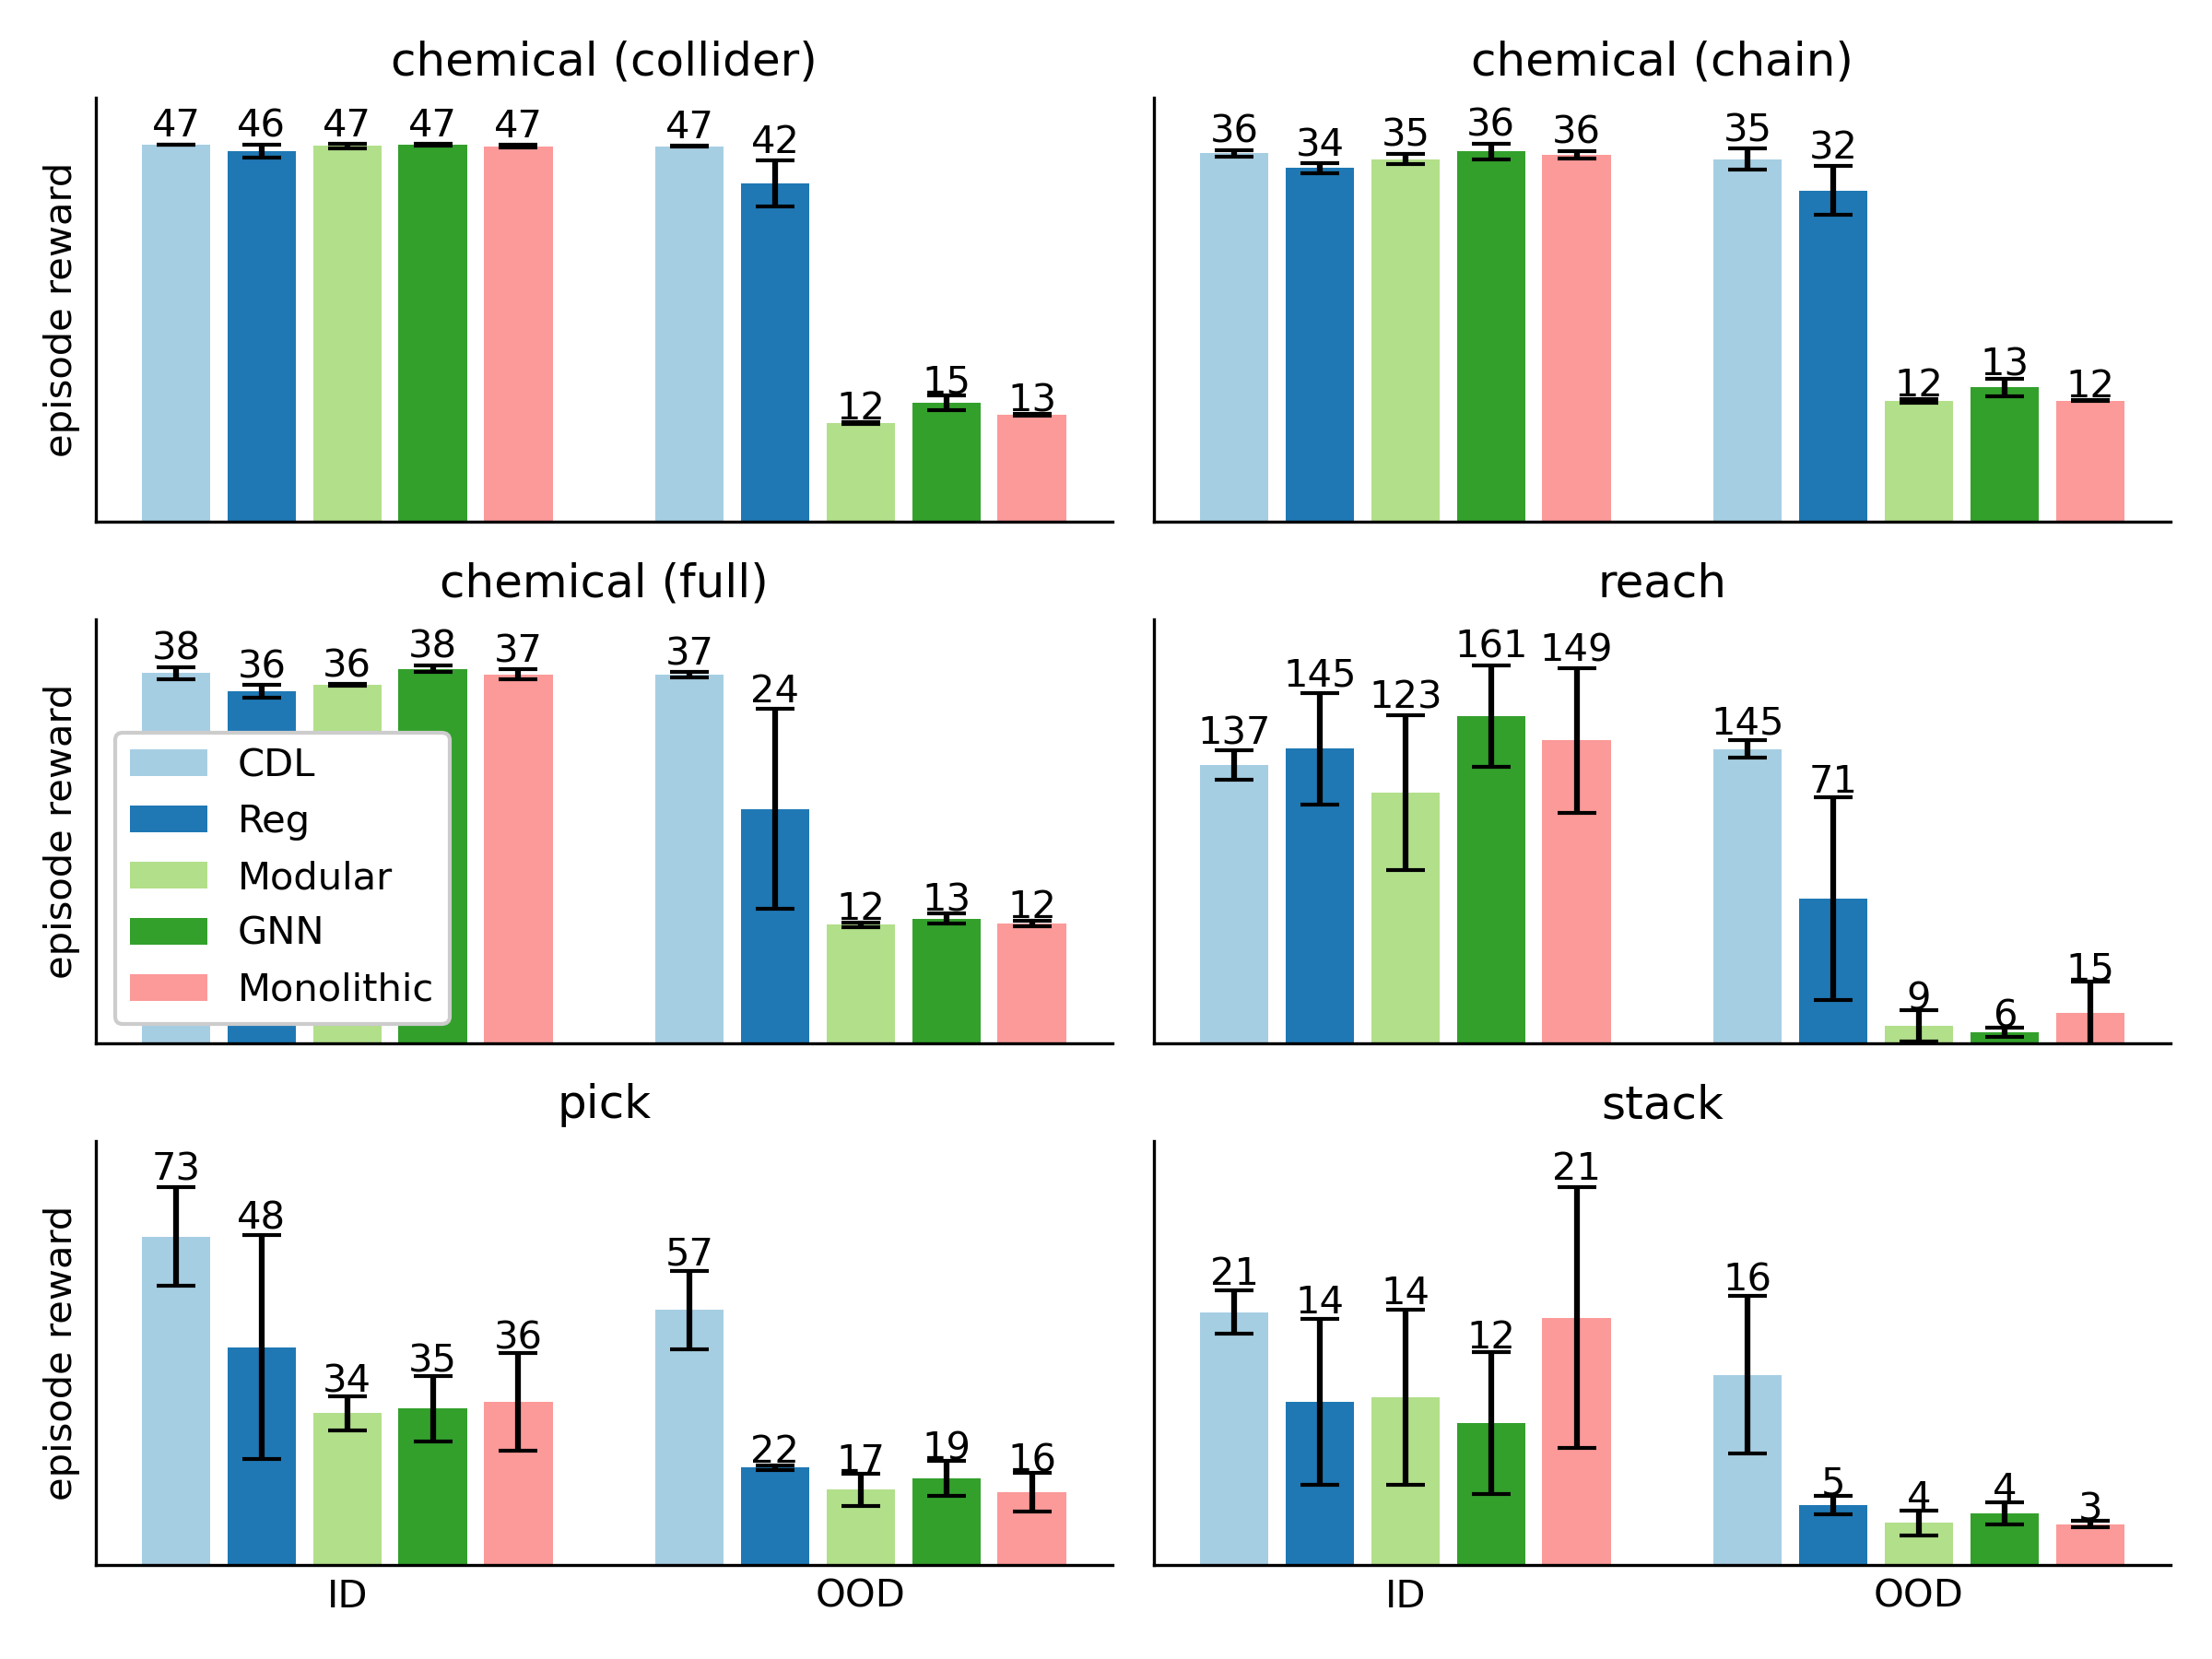
\includegraphics[width=1.0\columnwidth]{contents/figures/task_generalization.png}
  \vspace{-25pt}
  \caption{\small Episode reward of learned policies on ID and OOD states.}
  \label{fig:task_generalization}
  \vspace{-15pt}
\end{figure}

Furthermore, to test the generalization of the learned policies, we evaluate their performance for 100 episodes on both ID and OOD states, as shown in Fig. \ref{fig:task_generalization}. Again, \textsc{cdl} generalizes the best across all methods on OOD states.
